\documentclass[tikz]{standalone}
\usepackage{fourier}
\usetikzlibrary{arrows.meta}
\usetikzlibrary{calc}
\tikzset{>=latex}
\definecolor{bookblue}{RGB}{0,173,239}
\definecolor{bookpink}{RGB}{236,0,140}
\definecolor{bookgreen}{RGB}{50,200,0}
\definecolor{bookbluearea}{RGB}{204,239,252}
\tikzstyle{blueline}=[draw=bookblue,line width=0.2mm]
\tikzstyle{pinkline}=[draw=bookpink,line width=0.2mm]
\tikzstyle{greenline}=[draw=bookgreen,line width=0.2mm]
\tikzstyle{blackline}=[draw=black,line width=0.2mm]
\tikzstyle{bluearea}=[fill=bookbluearea]

\begin{document}
  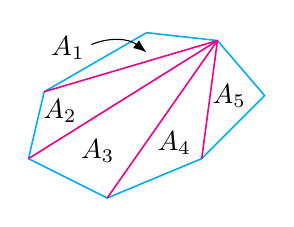
\begin{tikzpicture}
  \coordinate (A) at (0,0);
  \coordinate (B) at (1.2,0.5);
  \coordinate (C) at (2,1.3);
  \coordinate (D) at (1.4,2);
  \coordinate (E) at (.5,2.1);
  \coordinate (F) at (-0.8,1.35);
  \coordinate (G) at (-1,0.5);
  
  \draw[blueline] (A)--(B)--(C)--(D)--(E)--(F)--(G)--cycle;
  \draw[pinkline] (D) -- (A);
  \draw[pinkline] (D) -- (B);
  \draw[pinkline] (D) -- (F);
  \draw[pinkline] (D) -- (G);
  
  \node at (-0.50,1.9)   {$A_1$};
  \node at (-0.60,1.1)   {$A_2$};
  \node at (-0.12,0.6)   {$A_3$};
  \node at ( 0.85,0.7)   {$A_4$};
  \node at ( 1.55,1.3)   {$A_5$};
  
  \path[->,-Latex] (-0.2,1.95) edge [bend left=30] (0.5,1.85);
  
  \end{tikzpicture}
\end{document}